% %% %%%%%%%%%%%%%%%%%%%%%%%%%%%%%%%%%%%%%%%%%%%%%%%%%%%%%%%%%%
% intro.tex
%
% Author:  Mauricio Matamoros
% License: MIT
%
% %% %%%%%%%%%%%%%%%%%%%%%%%%%%%%%%%%%%%%%%%%%%%%%%%%%%%%%%%%%%

%!TEX root = ../practica.tex
%!TEX root = ../references.bib

\section{Introducción}%
\label{sec:introduction}
La presente práctica resume los pasos a seguir para desplegar texto en una pantalla de cristal líquido de 16 caracteres en dos líneas, mejor conocido como display LCD \(16\times2\).
En particular, se interesa en el desplegado de una cadena de más de 16 caracteres en la primera ĺínea del display y en la segunda la temperatura registrada por un sensor DS18B20 mediante el bus 1-Wire.

% %% %%%%%%%%%%%%%%%%%%%%%%%%%%%%%%%%%%%%%%%%%%%%%%%%%%%%%%%%%%
% intro-iic.tex
%
% Author:  Mauricio Matamoros
% License: MIT
%
% %% %%%%%%%%%%%%%%%%%%%%%%%%%%%%%%%%%%%%%%%%%%%%%%%%%%%%%%%%%%

%!TEX root = ../practica.tex
%!TEX root = ../references.bib

\subsection{Bus 1-Wire}%
\label{sec:intro-1wire}

\begin{wrapfigure}{r}{0.3\columnwidth}
	\centering
	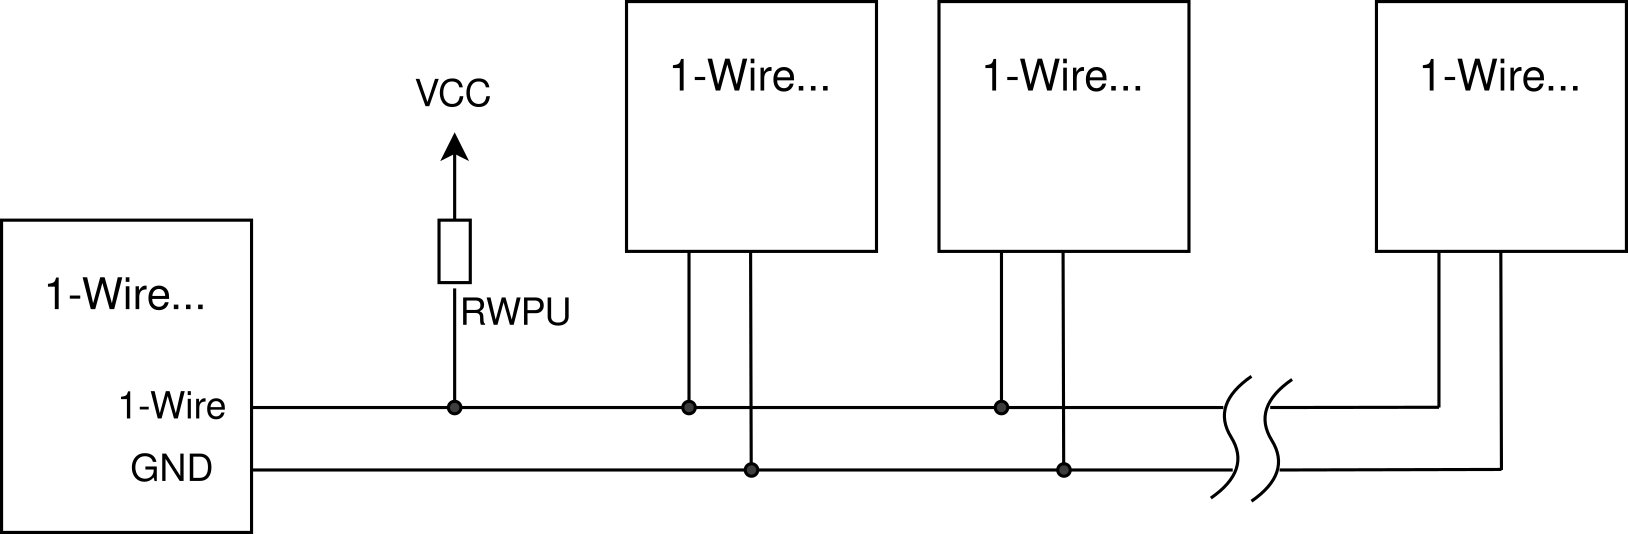
\includegraphics[width=0.3\columnwidth]{img/1-Wire.png}
	\caption{Bus 1-Wire con esclavos parásitos}%
	\label{fig:1wire-bus}
\end{wrapfigure}
1-Wire es un protocolo serial inventado por Dallas Semiconductor y diseñado para conectar dispositivos de muy baja velocidad mediante una interfaz de un sólo hilo (\Cref{fig:iic-bus}) para transmisión datos.
El bus 1-Wire es popular en meteorología (mediciones de temperatura, humedad y presión) debido a su facilidad de uso, fácil configuración y largo alcance (hasta 500 mestros)~\Citep{1WireWeb,Macekova20121}.

La transferencia de datos es serial asíncrona y transmite paquetes de 8 bits con velocidades de hasta 16.3 kbit/s y un voltaje variable entre 2.8V y 5.25V.
El dispositivo maestro, llamado MicroLAN, negocia la velocidad con los dispositivos esclavos y coordina la transmisión de datos.
Cada dispositivo esclavo es identificado mediante un paquete de 64 bits único y definido por el fabricante, donde los 8 bits más significativos especifican la familia del producto, es decir su tipo y función.
Además, la baja velocidad de operación del bus permite que el bus opere en modo \emph{parásito} con tan sólo dos hilos: datos y tierra. Esto se logra mediante la inclusión de un capacitor de 800pF que almacena energía cuando el bus de datos está activo~\Citep{1WireWeb,Macekova20121}.

Al ser un sensor completamente digital con un protocolo de transmisión de datos predefinido la lectura de datos del bus 1-Wire requiere de un controlador, mismo que viene integrado en la Raspberry Pi.
Una vez habilitado dicho controlador, éste enumerará todos los dispositivos conectados al bus 1-Wire, mismos que serán visibles bajo \texttt{/sys/bus/w1/devices}.

% %% %%%%%%%%%%%%%%%%%%%%%%%%%%%%%%%%%%%%%%%%%%%%%%%%%%%%%%%%%%
% intro-iic.tex
%
% Author:  Mauricio Matamoros
% License: MIT
%
% %% %%%%%%%%%%%%%%%%%%%%%%%%%%%%%%%%%%%%%%%%%%%%%%%%%%%%%%%%%%

%!TEX root = ../practica.tex
%!TEX root = ../references.bib

\subsection{Bus \IIC}%
\label{sec:intro-i2c}

\begin{wrapfigure}{r}{0.3\columnwidth}
	\centering
	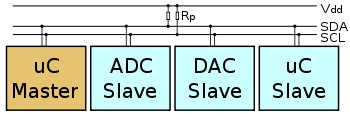
\includegraphics[width=0.3\columnwidth]{img/i2c-bus.png}
	\caption{Bus \IIC}%
	\label{fig:iic-bus}
\end{wrapfigure}
\IIC{} es un protocolo serial inventado por Phillips y diseñado para conectar dispositivos de baja velocidad mediante interfaces de dos hilos (\Cref{fig:iic-bus}).
El protocolo permite un número virtualmente ilimitado de dispositivos interconectados donde más de uno puede ser un dispositivo maestro.
El bus I2C es popular debido a su facilidad de uso y fácil configuración.
Sólo es necesario definir la velocidad máxima del bus, que está conformado por dos cables con resistencias pull-up~\Citep{IICWeb}.

\IIC{} utiliza solamente dos cables: SCL (reloj) y SDA (datos).
La transferencia de datos es serial y transmite paquetes de 8 bits con velocidades de hasta 5MHz.
Además, es requisito que cada dispositivo esclavo tenga una dirección de 7 bits que (el bit más significativo se utiliza para indicar si el paquete es una lectura o una escritura) debe ser única en el bus.
Los dispositivos maestros no necesitan dirección ya que estos generan la señal de reloj y coordinan a los dispositivos esclavos~\Citep{IICWeb}.

% CHKTEX-FILE 1
% CHKTEX-FILE 36
% CHKTEX-FILE 46

\newcommand{\ENA}{$\overline{\mbox{\texttt{\textsc{Ena}}}}$}
\newcommand{\RW}{\texttt{R}$\overline{\mbox{\texttt{W}}}$}
\newcommand{\RS}{\texttt{R}$\overline{\mbox{\texttt{S}}}$}
\newcommand{\hex}[1]{$0\times#1$}

\subsection{LCD 1602 \IIC{}}%
\label{sec:intro-lcd1602}

El LCD 1602 es un display de cristal líquido de 32 caracteres organizados en 2 líneas de 16 caracteres con iluminación trasera que cuenta con 8 pines de datos que pueden ser usados en modo de byte completo o por \emph{nibbles} (dos segmentos de 4 bits).

La inicialización del display usando los pines de datos no es tarea trivial.
Por facilidad, es común acoplar el display a un adaptador de puerto paralelo cuasi bidireccional con interfaz \IIC{}:\,el integrado PCF8574.
Este integrado  se encarga de la escritura de los datos al display LCD $16\times02$, permitiendo su uso mediante \IIC{}.

\medskip

\noindent \textbf{IMPORTANTE:} Normalmente el PCF8574 está preconfigurado con las direcciones \IIC{} \hex{3F} o \hex{27}.
Es crucial identificar correctamente la dirección \IIC{} del adaptador o el display no funcionará correctamente.

\subsubsection{Comunicación}

La comunicación con el LCD 1602 se realiza mediante la lectura y escritura de la memoria del display o el envío de comandos.
Como el display está conectado al PCF8574 que sólo tiene 8 pines, el display no puede ser operado en modo de byte completo pues no habría manera de enviar las 3 señales de control que el display requiere para operar:
\ENA{}, \RW{} y \RS{}.
Las señales de control operan como sigue:

\begin{table}[H]
	\centering
	\caption{Señales de control del LCD 1601}%
	\label{tbl:lcd-control-signals}
	\begin{tabularx}{0.9\linewidth}{c X}
		\toprule
		\multicolumn{1}{c}{\bfseries Señal} &
		\multicolumn{1}{c}{\bfseries Descripción} \\
		\midrule
		\ENA{} & Habilita el display. Poner esta línea en alto pone al LCD 1602 en modo de bajo consumo. \\

		\RW{}  & Establece que la operación es una lectura (alto) o una escritura (bajo) de la memoria del display. \\

		\RS{}  & Establece si la información enviada debe ser interpretada como datos (alto) o como un comando para el display (bajo). \\
		\bottomrule
	\end{tabularx}
\end{table}

Al haber sólo 4 bits disponibles, el envío de datos y de comandos requerirá de dos operaciones de escritura en el bus \IIC{}: el primero para la parte alta o nibble superior y el segundo para la parte baja o nibble inferior.

Los \Cref{alg:lcd-command-send,alg:lcd-data-send} resumen el envío de datos y comandos.
Ambos algoritmos son, escencialmente, idénticos, con la única diferencia de un cambio de valor en la bandera \RS{}.

\begin{algorithm}[H]
	\centering
	\caption{Envío de commandos al LCD 1601}%
	\label{alg:lcd-command-send}
	\begin{algorithmic}
		\Procedure{SendCommand}{cmd}
			\State buffer $\leftarrow$ cmd \& \hex{f0}
			\Comment{Elimina el nibble inferior}

			\State buffer $\leftarrow$ buffer $\vert$ \hex{04}
			\Comment{Banderas \ENA{}$=1$, \RW{}$=0$, \RS{}$=0$}

			\State \Call{SendWord}{\texttt{LCD\_ADDR}, buffer}
			\Comment{Envía bits 7--4}

			\State \Call{Sleep}{2ms}
			\Comment{Tiempo de espera del display}

			\State buffer $\leftarrow$ buffer \& \hex{FB}
			\Comment{Cambia bandera \ENA{}$=0$}

			\State \Call{SendWord}{\texttt{LCD\_ADDR}, buffer}
			\Comment{Envía confirmación de fin de nibble}

			\medskip

			\State buffer $\leftarrow$ (cmd \& \hex{f0}) $\ll$ 4
			\Comment{Elimina el nibble superior y recorre el inferior a la parte alta}

			\State buffer $\leftarrow$ buffer $\vert$ \hex{04}
			\Comment{Banderas \ENA{}$=1$, \RW{}$=0$, \RS{}$=0$}

			\State \Call{SendWord}{\texttt{LCD\_ADDR}, buffer}
			\Comment{Envía bits 3--0}

			\State \Call{Sleep}{2ms}
			\Comment{Tiempo de espera del display}

			\State buffer $\leftarrow$ buffer \& \hex{FB}
			\Comment{Cambia bandera \ENA{}$=0$}

			\State \Call{SendWord}{\texttt{LCD\_ADDR}, buffer}
			\Comment{Envía confirmación de fin de nibble}
		\EndProcedure{}
	\end{algorithmic}
\end{algorithm}

\begin{algorithm}[H]
	\centering
	\caption{Envío de datos al LCD 1601}%
	\label{alg:lcd-data-send}
	\begin{algorithmic}
		\Procedure{SendData}{data}
			\State buffer $\leftarrow$ data \& \hex{f0}
			\Comment{Elimina el nibble inferior}

			\State buffer $\leftarrow$ buffer $\vert$ \hex{05}
			\Comment{Banderas \ENA{}$=1$, \RW{}$=0$, \RS{}$=0$}

			\State \Call{SendWord}{\texttt{LCD\_ADDR}, buffer}
			\Comment{Envía bits 7--4}

			\State \Call{Sleep}{2ms}
			\Comment{Tiempo de espera del display}

			\State buffer $\leftarrow$ buffer \& \hex{FB}
			\Comment{Cambia bandera \ENA{}$=0$}

			\State \Call{SendWord}{\texttt{LCD\_ADDR}, buffer}
			\Comment{Envía confirmación de fin de nibble}

			\medskip

			\State buffer $\leftarrow$ (data \& \hex{f0}) $\ll$ 4
			\Comment{Elimina el nibble superior y recorre el inferior a la parte alta}

			\State buffer $\leftarrow$ buffer $\vert$ \hex{05}
			\Comment{Banderas \ENA{}$=1$, \RW{}$=0$, \RS{}$=0$}

			\State \Call{SendWord}{\texttt{LCD\_ADDR}, buffer}
			\Comment{Envía bits 3--0}

			\State \Call{Sleep}{2ms}
			\Comment{Tiempo de espera del display}

			\State buffer $\leftarrow$ buffer \& \hex{FB}
			\Comment{Cambia bandera \ENA{}$=0$}

			\State \Call{SendWord}{\texttt{LCD\_ADDR}, buffer}
			\Comment{Envía confirmación de fin de nibble}
		\EndProcedure{}
	\end{algorithmic}
\end{algorithm}

La función \texttt{\textsc{SendWord}} se presenta a continuación en lenguage Python. Esta dependerá de la implementación subyaciente de \texttt{smbus2}.

\begin{lstlisting}[language=Python]
import smbus2
BUS = smbus2.SMBus(1)
def send_word(addr, data):
	global BLEN
	temp = data
	if BLEN == 1:
		temp |= 0x08
	else:
		temp &= 0xF7
	BUS.write_byte(addr ,temp)
\end{lstlisting}

\subsubsection{Inicialización}
\noindent
La rutina de inicialización del LCD 1602 es la siguiente:

\begin{algorithm}[H]
	\centering
	\caption{Inicialización del LCD 1601}%
	\label{tbl:lcd-init}
	\begin{algorithmic}
		\Procedure{InitLCD}{}
			\State \Call{SendCommand}{\hex{33}}
			\Comment{Inicializar display}
			\State \Call{Sleep}{5ms}

			\State \Call{SendCommand}{\hex{32}}
			\Comment{Cambiar a modo de 4 líneas}
			\State \Call{Sleep}{5ms}

			\State \Call{SendCommand}{\hex{28}}
			\Comment{Configurar modo: 2 líneas y caracteres de 35 puntos}
			\State \Call{Sleep}{5ms}

			\State \Call{SendCommand}{\hex{0C}}
			\Comment{Habilitar display y ocultar cursor}
			\State \Call{Sleep}{5ms}

			\State \Call{SendCommand}{\hex{01}}
			\Comment{Borrar pantalla}
			\State \Call{Sleep}{5ms}
		\EndProcedure{}
	\end{algorithmic}
\end{algorithm}
\medskip

Nótese la espera activa de 5ms después de cada comando. Esta espera es para dar tiempo al display de cambiar de modo, ya que la inicialización es un proceso lento.

\subsubsection{Comandos}
Los comandos del LCD 1602 son los siguientes.

\begin{tabularx}{0.9\linewidth}{c X}
	\toprule
	\multicolumn{1}{c}{\bfseries Comando} &
	\multicolumn{1}{c}{\bfseries Descripción} \\
	\midrule
	\hex{01} & Borrar pantalla \\
	\hex{08} & Activar luz posterior \\
	\hex{0C} & Habilitar display sin cursor \\
	\hex{33} & Inicializar display (modo de 8 pines) \\
	\hex{32} & Cambio a modo de 4 pines \\
	\hex{32} & Configurar display con 2 líneas y caracteres de $5\times7$ puntos \\
	\hex{80} + \hex{40}$\times y + x$
	         & Mover cursor a posición $(x, y)$\\
	\bottomrule
\end{tabularx}

